%%%%%%%%%%%%%%%%%%%%%%%%%%%%%%%%%%%%%%%%%
% LaTeX Template
% http://www.LaTeXTemplates.com
%
% Original author:
% Linux and Unix Users Group at Virginia Tech Wiki
% (https://vtluug.org/wiki/Example_LaTeX_chem_lab_report)
%
% License:
% CC BY-NC-SA 3.0 (http://creativecommons.org/licenses/by-nc-sa/3.0/)
%
%%%%%%%%%%%%%%%%%%%%%%%%%%%%%%%%%%%%%%%%%

%----------------------------------------------------------------------------------------
%	PACKAGES AND DOCUMENT CONFIGURATIONS
%----------------------------------------------------------------------------------------

\documentclass[12pt]{article}
\usepackage{geometry} % Pour passer au format A4
\geometry{hmargin=1cm, vmargin=1cm} %

\usepackage{graphicx} % Required for including pictures
\usepackage{float} %

%Français
\usepackage[T1]{fontenc}
\usepackage[english,francais]{babel}
\usepackage[utf8]{inputenc}
\usepackage{eurosym}
\usepackage{lmodern}
\usepackage{url}
\usepackage{multicol}

%Maths
\usepackage{amsmath,amsfonts,amssymb,amsthm}
%\usepackage[linesnumbered, ruled, vlined]{algorithm2e}
%\SetAlFnt{\small\sffamily}

%Autres
\linespread{1} % Line spacing
\setlength\parindent{0pt} % Removes all indentation from paragraphs

\pagestyle{empty}
\usepackage{lastpage}
\usepackage{fancyhdr} % Custom headers and footers
\pagestyle{fancyplain} % Makes all pages in the document conform to the custom headers and footers

\fancyfoot[C]{} % Page numbering for right footer
\fancyfoot[R]{\vspace{-1cm}\thepage / \pageref{LastPage}} % Page numbering for right footer



\renewcommand{\labelenumi}{\alph{enumi}.} %

%----------------------------------------------------------------------------------------
%	DOCUMENT INFORMATION
%----------------------------------------------------------------------------------------
\begin{document}

\setlength{\columnseprule}{0pt}

\section*{EXERCICE 1 (6 pts) } % barème sur .

En électronique on utilise la fonction de transfert $\mathcal{H}$ définie pour une pulsation $x > 0$ par :
$$\mathcal{H}(x) = \frac{ix}{2x + i}$$
$i$ étant le nombre complexe de module $1$ et d'argument $\dfrac{\pi}{2}$.

\subsection*{Cas particulier}

\begin{enumerate}
\item[1.]
  \begin{enumerate}
  \item[a.] Déterminer la forme algébrique du nombre complexe $\mathcal{H}(1)$ .
  \item[b.] Déterminer le module et un argument de $\mathcal{H}\left(\dfrac{1}{2} \right)$. Donner alors la forme exponentielle du nombre complexe $\mathcal{H}\left(\dfrac{1}{2} \right)$.
  \end{enumerate}
\end{enumerate}

\subsection*{Cas Général}

\begin{enumerate}
\item[2.] Montrer que $\mathcal{H}(x) = \dfrac{x}{1 + 4x^2} +  i \dfrac{2x^2}{1 + 4x^2} $.
\item[3.] On pose $\theta (x)$ un argument du nombre complexe $\mathcal{H}(x)$ ; $\theta(x)$ est appelé \textit{phase du circuit}.

  \begin{enumerate}
  \item[a.] Montrer que $\theta(x) = arctan(2x)$.
  \item[b.] Déterminer la pulsation $x$ pour que la phase du circuit soit égale à $\dfrac{\pi}{6}$.
  \item[c.] Étudier les variations de la fonction $\theta$ sur $I = [ 0 ; +\infty [$.
    \item[d.] Étudier les limites de la fonction $\theta$ aux bornes de l'intervalle I. Conséquence graphique ?
    \item[e.] Tracer la représentation graphique de $\theta$ dans le repère ci-joint en annexe.
  \end{enumerate}

\end{enumerate}

\newpage
\section*{EXERCICE 2 (3.5 pts) } % barème sur .

\begin{multicols}{2}
  \begin{enumerate}
  \item[1.]
    Soit la fonction numérique $g$ définie sur $[0 ; \pi]$ par $g(t) = (1 + \cos^{2}(t)) \sin^{2}(t)$.\\ \vspace{0.5cm}\\
    À l'aide du graphe de $g'$ représenté FIGURE 1, \\
    déterminer le signe de $g'(t)$ et déduire le tableau de variation de $g$.

  \item[2.] Voici la courbe représentative de g
  
  \end{enumerate}

  \begin{figure}[H]
    \centering
    \fbox{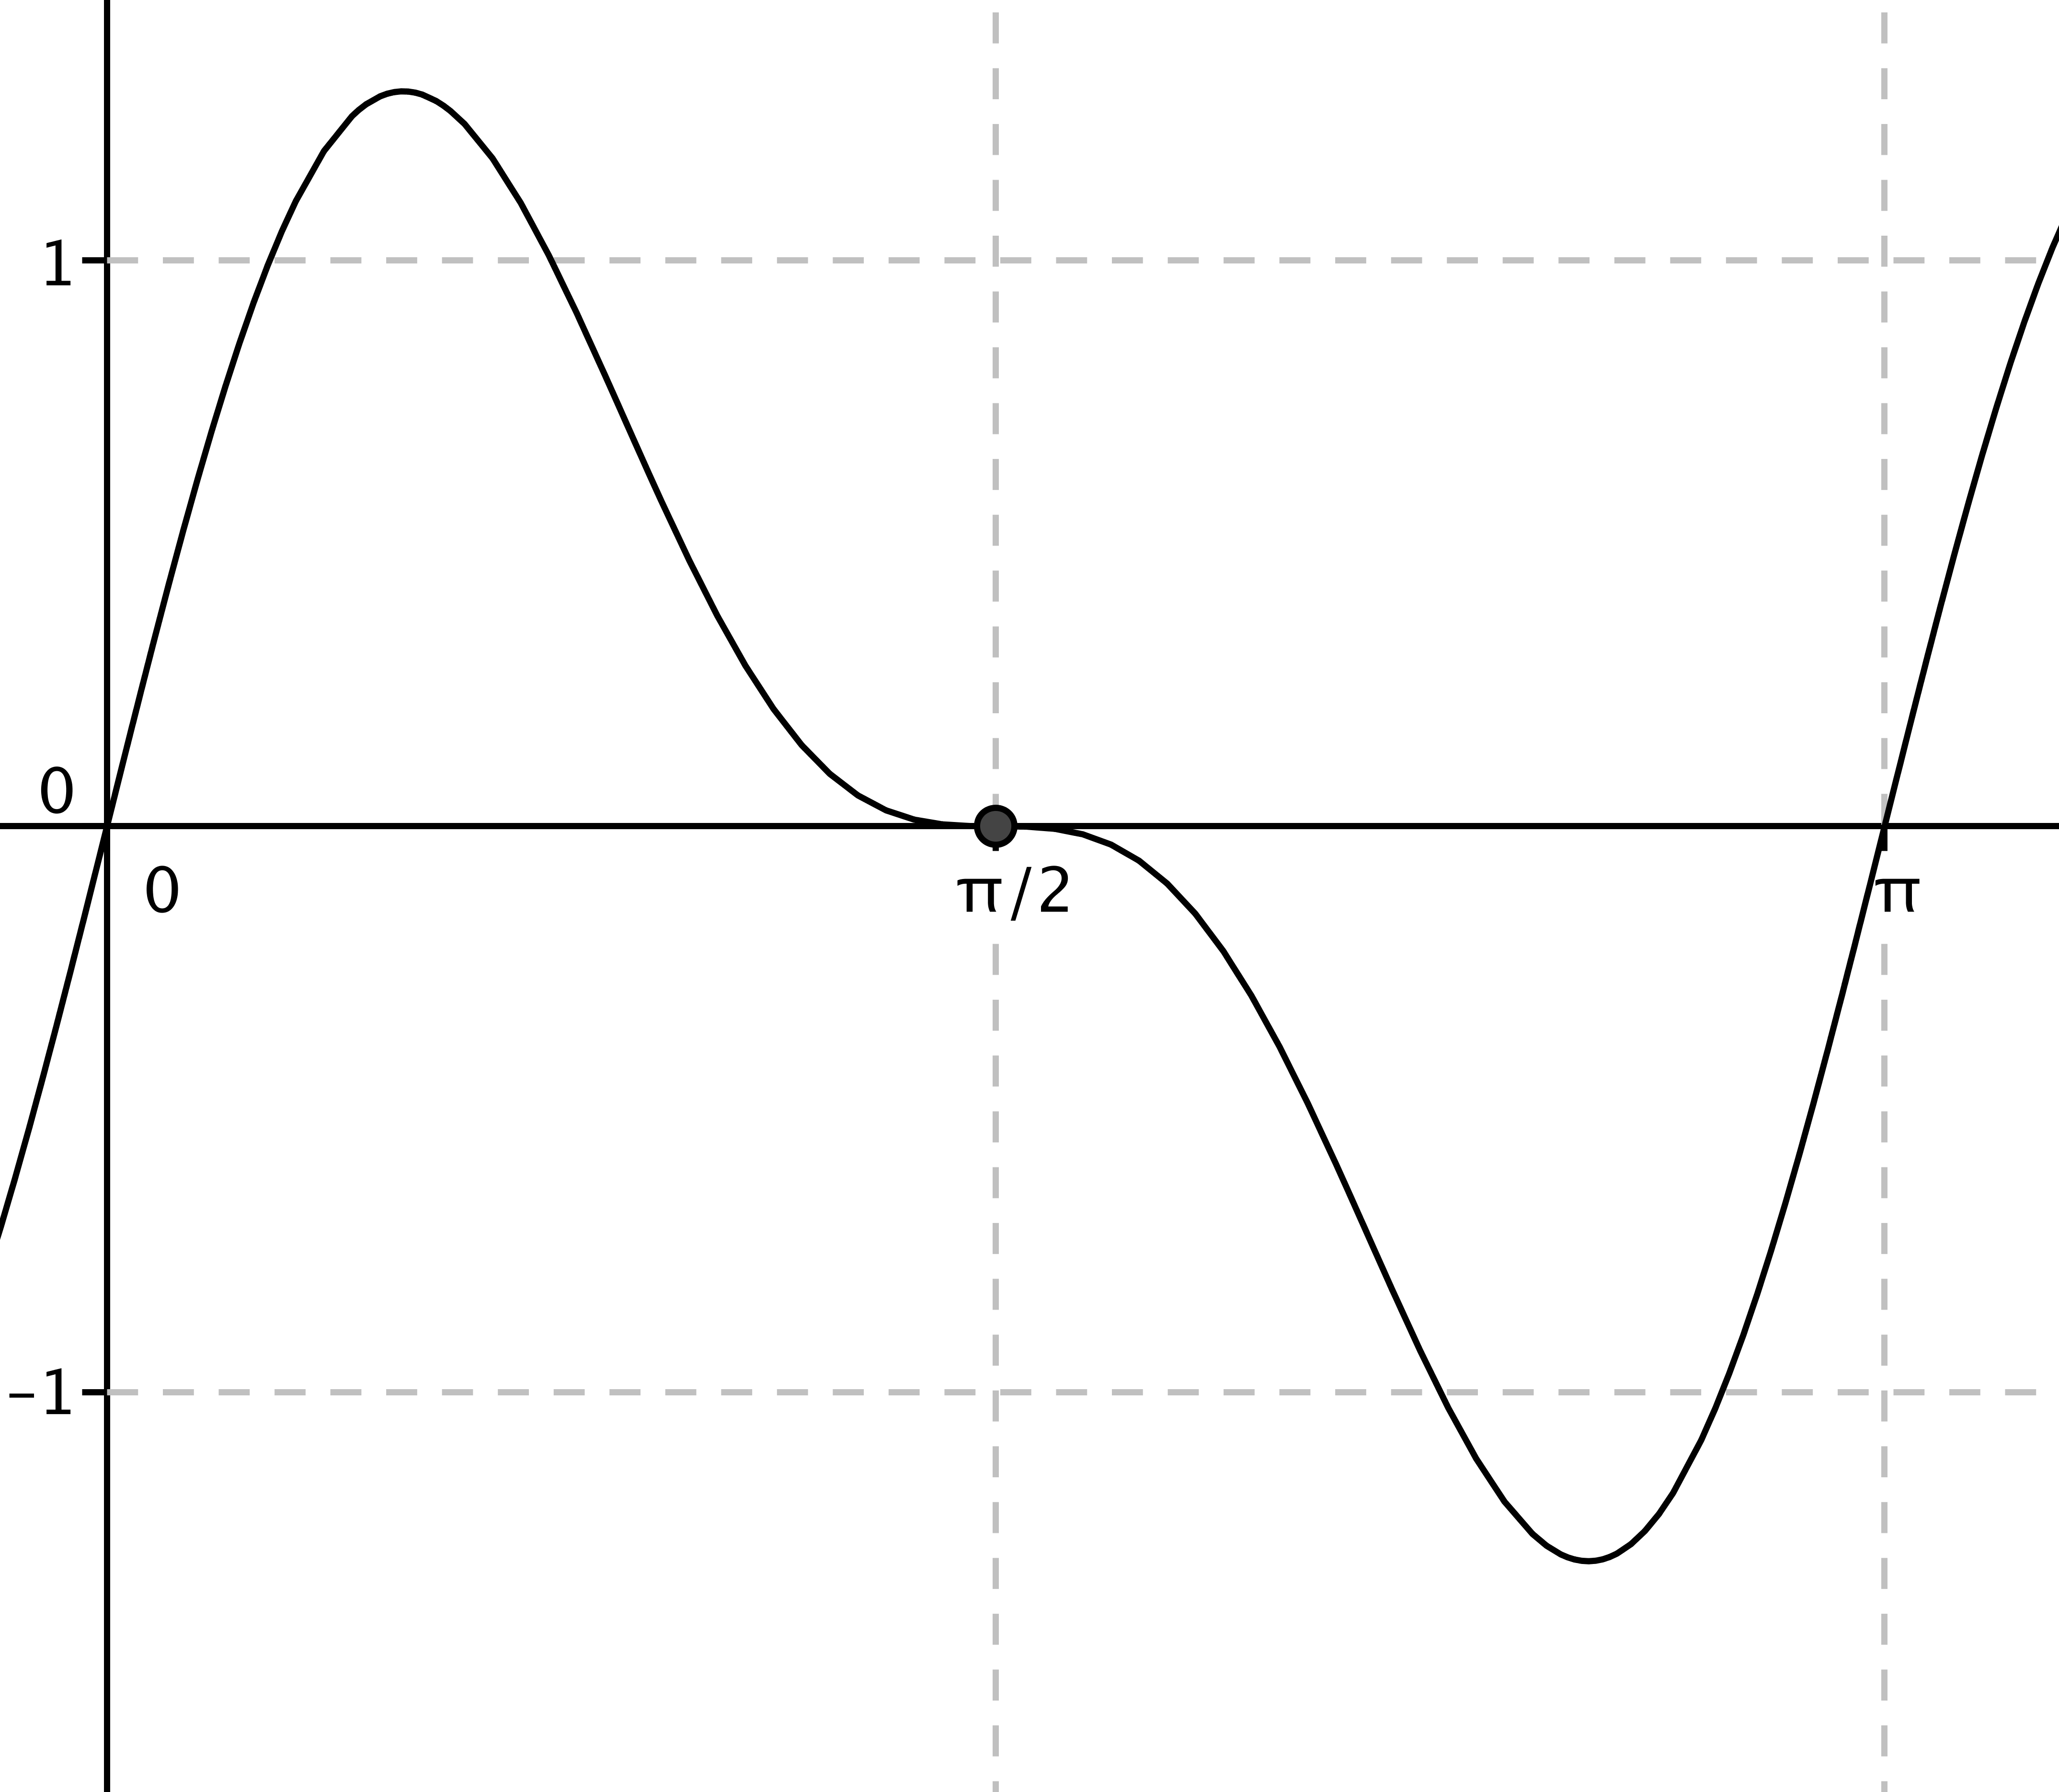
\includegraphics[width=0.3\textwidth]{img/exo2-1.png}}
    \caption{$g'$}
  \end{figure}
\end{multicols}

  \begin{figure}[H]
    \centering
    \fbox{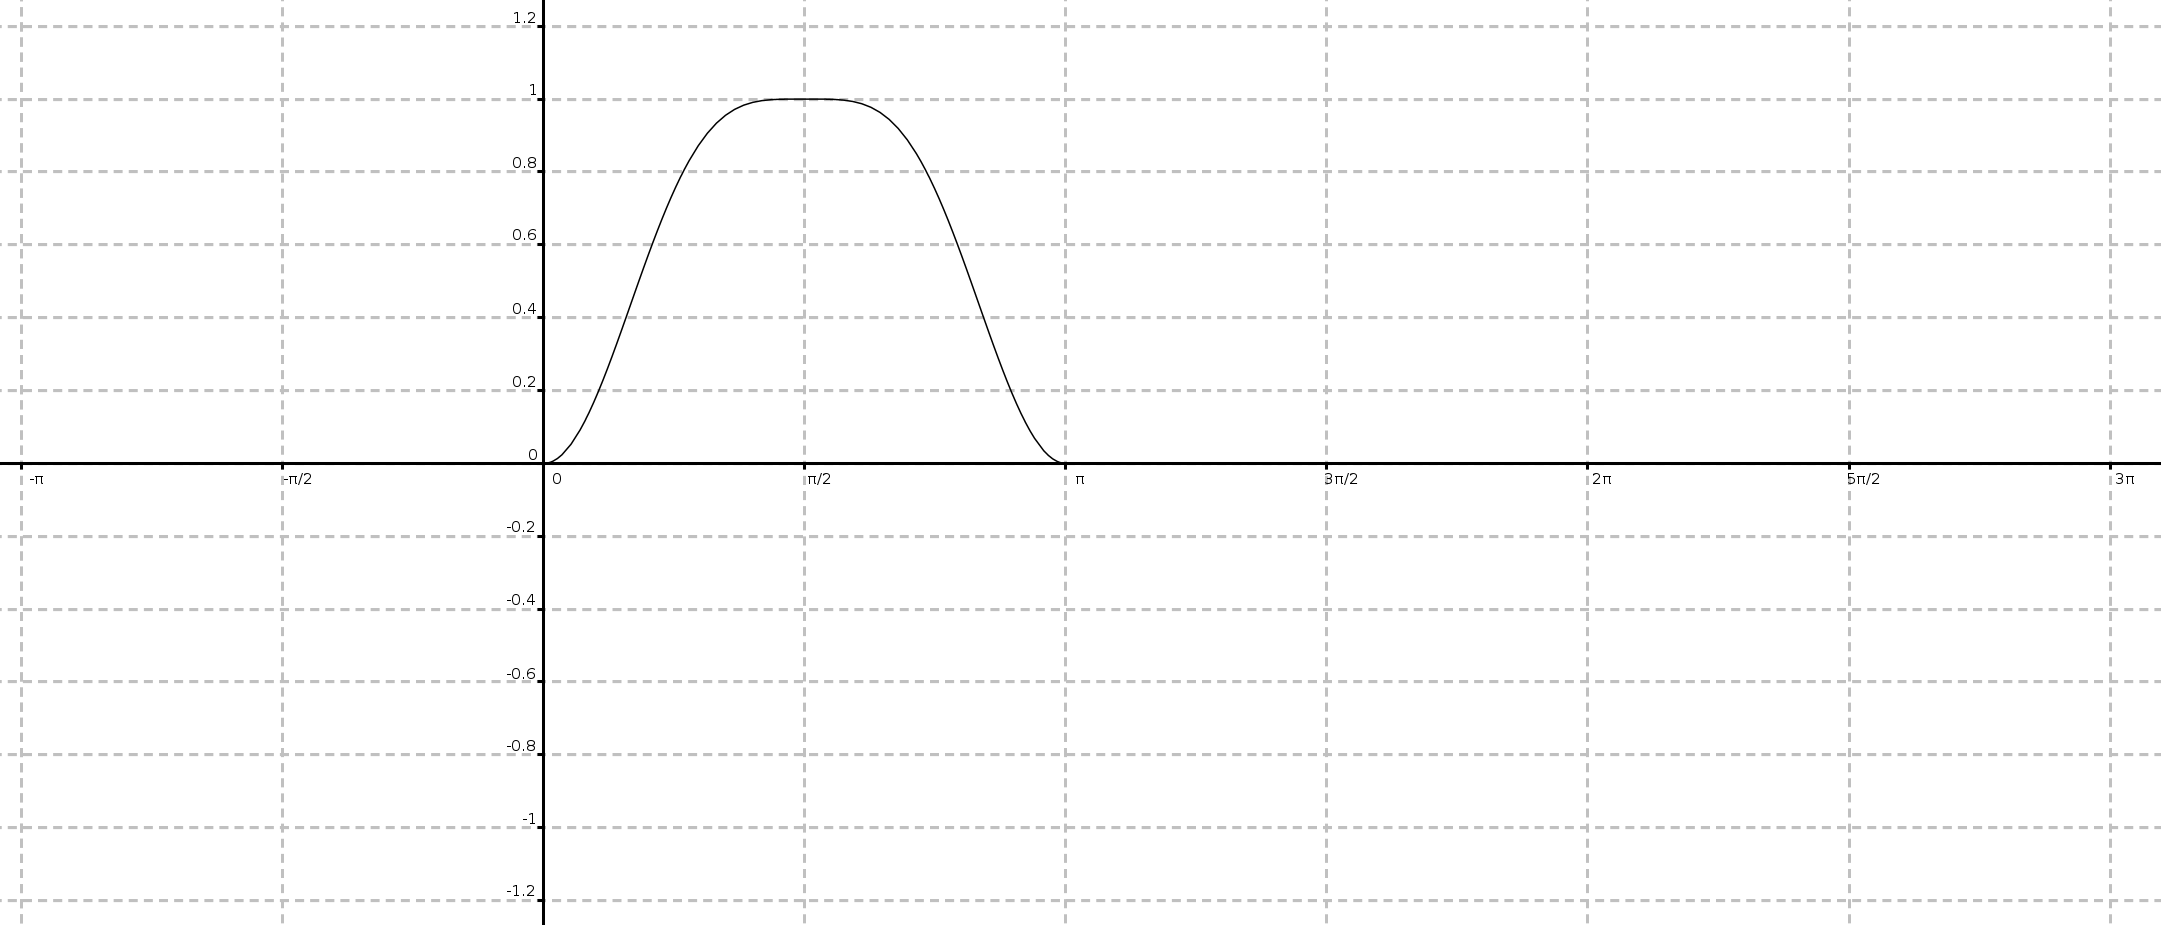
\includegraphics[width=0.65\textwidth]{img/exo2-2.png}}
    \caption{Courbe représentative de $g$}
  \end{figure}

  On considère maintenant la fonction $h$ définie sur $\mathbb{R}$ telle que $h$ est impaire, $2\pi$-périodique et définie par :
  $$h(t) = g(t) \text{ si } t \in [0 ; \pi ]$$

  Tracer la courbe représentative de $h$ sur $[-\pi ; 3\pi ]$ . Faire le tracer sur la FIGURE 2.

\section*{EXERCICE 3 (3.5 pts) } % barème sur .

\begin{multicols}{2}

  \begin{figure}[H]
    \centering
    \fbox{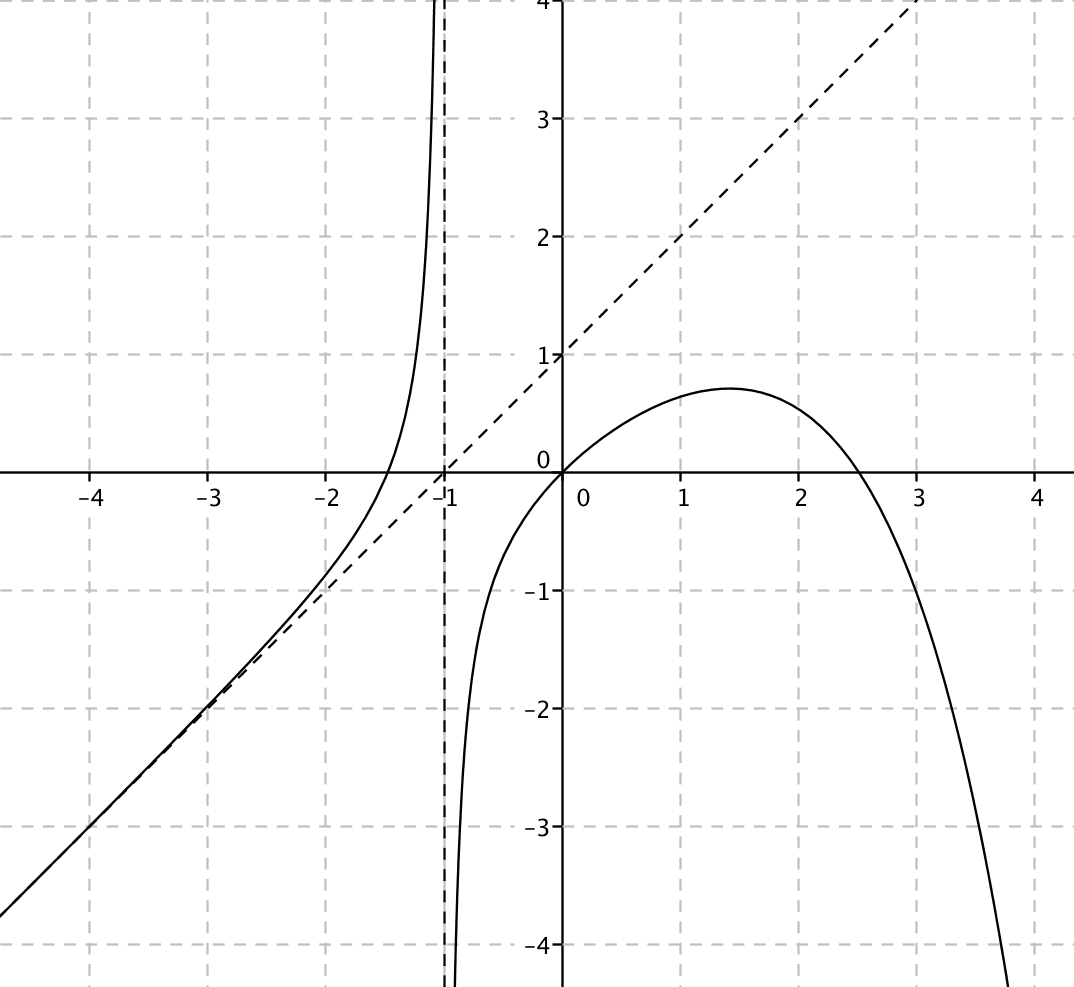
\includegraphics[width=0.4\textwidth]{img/exo3.png}}
  \end{figure}

  Voici la courbe représentative d'une fonction $f$ ainsi que 2 droites asymptotes à la courbe.\\
  À l'aide des éléments graphiques :
  \begin{enumerate}
  \item[1.] Déterminer l'ensemble de définition de $f$.
  \item[2.] Donner l'équation des 2 asymptotes.
  \item[3.] Donner les limites de $f$ aux bornes de son intervalle de définition.
  \end{enumerate}
\end{multicols}

\newpage
\section*{EXERCICE 4 (7 pts) } % barème sur 7.

\subsection*{I - Étude d'une fonction auxiliaire}

Soit $g$ la fonction définie sur $] 0 ; + \infty [$ par $g(x) = 8 x^2 + 36 - 36 \ln(x)$.
      \begin{enumerate}
      \item[1.] Déterminer $g'$ la dérivée de $g$. 
      \item[2.] Étudier le signe de $g'(x)$ sur $] 0 ; + \infty [$. En déduire le tableau de variations de $g$ sur $] 0 ; + \infty [$.
    \item[3.] Chercher une valeur approchée de $g \left( \dfrac{3}{2} \right)$. En déduire le signe de $g(x)$ sur $] 0 ; + \infty [$.
      \end{enumerate}

      \subsection*{II - Étude d'une fonction f}
      Soit $f$ la fonction définie sur $] 0 ; + \infty [$ par $f(x) = 2x + 3 + \dfrac{9 \ln(x)}{x}$.
      On note $\mathcal{C}_f$ sa représentation graphique.

      \begin{enumerate}
      \item[1.] Calculer la limite de la fonction $f$ en $0$. Conséquence graphique ?
      \item[2.] Montrer que $\mathcal{C}_f$ admet la droite d'équation $y = 2x + 3$ comme asymptote en $+\infty$. On note $\mathcal{D}$ la représentation graphique de cette droite.
      \item[3.] Étudier la position relative de $\mathcal{C}_f$ par rapport à $\mathcal{D}$.
      \item[4.] Déterminer $f'(x)$, $f'$ étant la dérivée de $f$. Vérifier qu'on peut l'écrire $f'(x) = \dfrac{g(x)}{4x^2}$.
      \item[5.] En s'appuyant sur la question I-4., déduire le signe de $f'(x)$ et les variations de $f$ sur  $] 0 ; + \infty [$. 
      \end{enumerate}

      \noindent\hrulefill

      \section*{ANNEXE}

      \begin{figure}[h]
        \centering
        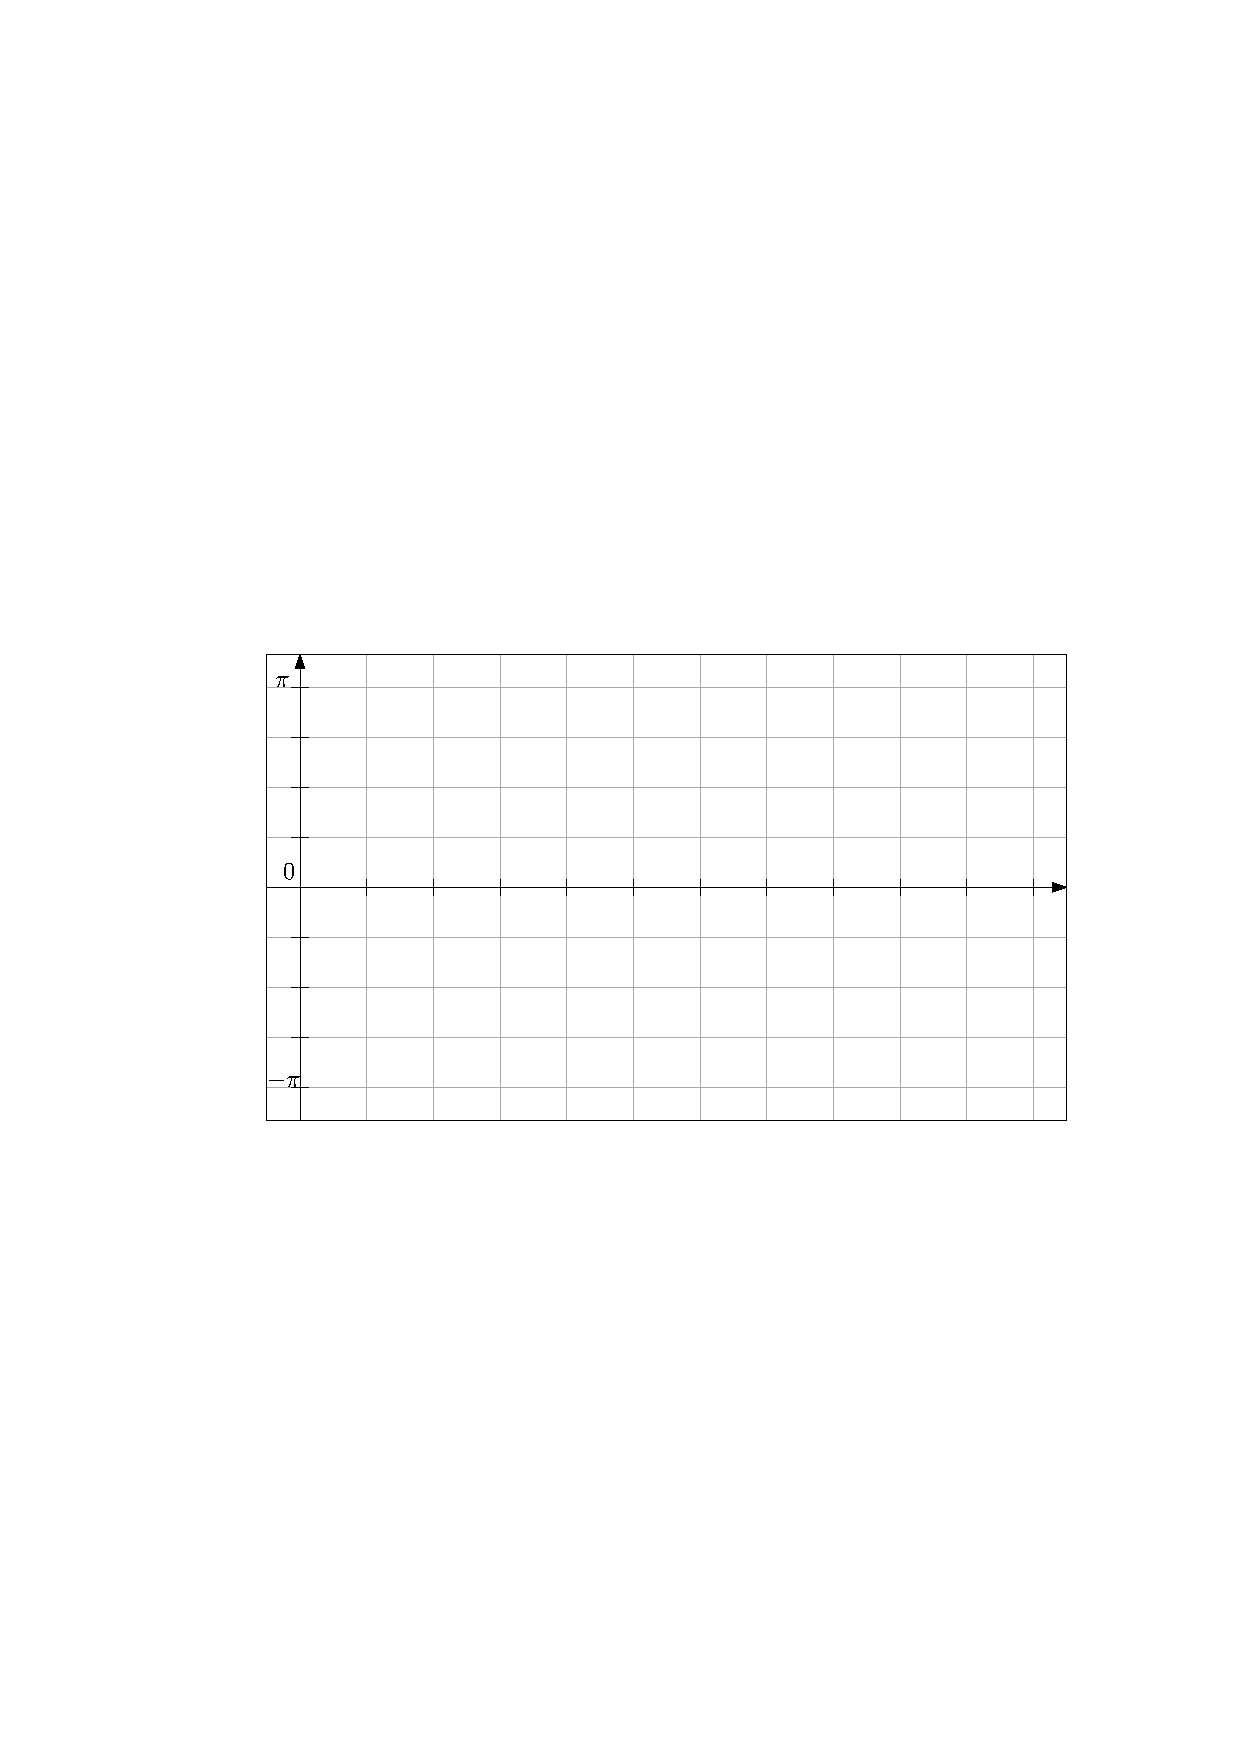
\includegraphics[width=0.9\textwidth]{sources/img/grille.pdf}
      \end{figure}

\end{document}
